\documentclass{article}

\usepackage{graphicx} % Required for inserting images
\usepackage[left=1in,right=1in,top=1in,bottom=1in]{geometry} \usepackage{amsmath}
\usepackage{amsthm} %proof environment
\usepackage{amsthm} %proof environment
\usepackage{amssymb}
\usepackage{amsfonts}
\usepackage{enumitem} %nice lists
\usepackage{verbatim} %useful for something 
\usepackage{xcolor}
\usepackage{setspace}
\usepackage{titlesec}
\usepackage{blindtext} % I have no idea what this is 
\usepackage{caption}  % need this for unnumbered captions/figures
\usepackage{natbib}
\usepackage{appendix}
\usepackage{tikz}
\usepackage{hyperref}


\hypersetup{
    colorlinks=true,
    linkcolor=blue,
    filecolor=magenta,      
    urlcolor=blue,
    pdftitle={Overleaf Example},
    pdfpagemode=FullScreen,
    }

\titleformat{\section}{\bfseries\Large}{Problem \thesection:}{5pt}{}

\begin{document}

\title{AM 260 - Computational Fluid Dynamis: Homework 3}
\author{Dante Buhl}


\newcommand{\wrms}{w_{\text{rms}}}
\newcommand{\bs}[1]{\boldsymbol{#1}}
\newcommand{\tb}[1]{\textbf{#1}}
\newcommand{\bmp}[1]{\begin{minipage}{#1\textwidth}}
\newcommand{\emp}{\end{minipage}}
\newcommand{\R}{\mathbb{R}}
\newcommand{\C}{\mathbb{C}}
\newcommand{\N}{\mathcal{N}}
%\newcommand{\K}{\bs{\mathrm{K}}}
\newcommand{\m}{\bs{\mu}_*}
\newcommand{\s}{\bs{\Sigma}_*}
\newcommand{\dt}{\Delta t}
\newcommand{\dx}{\Delta x}
\newcommand{\tr}[1]{\text{Tr}(#1)}
\newcommand{\Tr}[1]{\text{Tr}(#1)}
\newcommand{\Div}{\nabla \cdot}
\renewcommand{\div}{\nabla \cdot}
\newcommand{\Curl}{\nabla \times}
\newcommand{\Grad}{\nabla}
\newcommand{\grad}{\nabla}
\newcommand{\grads}{\nabla_s}
\newcommand{\gradf}{\nabla_f}
\newcommand{\xs}{x_s}
\newcommand{\x}{\bs{x}}
\newcommand{\xf}{x_f}
\newcommand{\ts}{t_s}
\newcommand{\tf}{t_f}
\newcommand{\pt}{\partial t}
\newcommand{\pz}{\partial z}
\newcommand{\uvec}{\bs{u}}
\newcommand{\bvec}{\bs{B}}
\newcommand{\nvec}{\hat{\bs{n}}}
\newcommand{\tu}{\tilde{\uvec}}
\newcommand{\B}{\bs{B}}
\newcommand{\A}{\bs{A}}
\newcommand{\jvec}{\bs{j}}
\newcommand{\F}{\bs{F}}
\newcommand{\T}{\tilde{T}}
\newcommand{\ez}{\bs{e}_z}
\newcommand{\ex}{\bs{e}_x}
\newcommand{\ey}{\bs{e}_y}
\newcommand{\eo}{\bs{e}_{\bs{\Omega}}}
\newcommand{\ppt}[1]{\frac{\partial #1}{\partial t}}
\newcommand{\pp}[2]{\frac{\partial #1}{\partial #2}}
\newcommand{\pptwo}[2]{\frac{\partial^2 #1}{\partial #2^2}}
\newcommand{\ddtwo}[2]{\frac{d^2 #1}{d #2^2}}
\newcommand{\DDt}[1]{\frac{D #1}{D t}}
\newcommand{\ppts}[1]{\frac{\partial #1}{\partial t_s}}
\newcommand{\pptf}[1]{\frac{\partial #1}{\partial t_f}}
\newcommand{\ppz}[1]{\frac{\partial #1}{\partial z}}
\newcommand{\ddz}[1]{\frac{d #1}{d z}}
\newcommand{\ppzetas}[1]{\frac{\partial^2 #1}{\partial \zeta^2}}
\newcommand{\ppzs}[1]{\frac{\partial #1}{\partial z_s}}
\newcommand{\ppzf}[1]{\frac{\partial #1}{\partial z_f}}
\newcommand{\ppx}[1]{\frac{\partial #1}{\partial x}}
\newcommand{\ddx}[1]{\frac{d #1}{d x}}
\newcommand{\ppxi}[1]{\frac{\partial #1}{\partial x_i}}
\newcommand{\ppxj}[1]{\frac{\partial #1}{\partial x_j}}
\newcommand{\ppy}[1]{\frac{\partial #1}{\partial y}}
\newcommand{\ppzeta}[1]{\frac{\partial #1}{\partial \zeta}}
\renewcommand{\k}{\bs{k}}
\newcommand{\real}[1]{\text{Re}\left[#1\right]}


\maketitle 
% This line removes the automatic indentation on new paragraphs
\setlength{\parindent}{0pt}

\section{Lax-Friedrichs Method}

\begin{enumerate}[label = (\alph*)]
    \item Show that the LW method is convergent if $|C_a| \le 1$. 

    \textbf{Consistency}
        Here are the taylor expansions which will be used to show consistency
        both for 1.a. and 2.a.
        \begin{align*}
            U_j^{n+1} &= U_j^n + \Delta t U_{t, j}^n + 
            \frac{\Delta t^2}{2}U_{tt, j}^n + \frac{\Delta t^3}{6}U_{ttt, j}^n
            + \frac{\Delta t^4}{24}U_{tttt, j}^n + O(\Delta t^5)\\
            U_{j+1}^{n} &= U_j^n + \Delta x U_{x, j}^n + 
            \frac{\Delta x^2}{2}U_{xx, j}^n + \frac{\Delta x^3}{6}U_{xxx, j}^n
            + \frac{\Delta x^4}{24}U_{xxxx, j}^n + O(\Delta x^5)\\
            U_{j-1}^{n} &= U_j^n - \Delta x U_{x, j}^n + 
            \frac{\Delta x^2}{2}U_{xx, j}^n - \frac{\Delta x^3}{6}U_{xxx, j}^n
            + \frac{\Delta x^4}{24}U_{xxxx, j}^n + O(\Delta x^5)
        \end{align*}
        \begin{align*}
            \Delta t E_{LT} &= 
            U_j^n + \Delta t U_{j, t}^n + \frac{\Delta t^2}{2} U_{j, tt}^n +
            \ldots \\
            &-\frac{1}{2}\left(U_j^n + \Delta x U_{j, x}^n + \frac{\Delta
            x^2}{2}U_{j, xx}^n + \ldots\right)\\
            &-\frac{1}{2}\left(U_j^n - \Delta x U_{j, x}^n + \frac{\Delta
            x^2}{2}U_{j, xx}^n + \ldots\right) \\
            &+\frac{a\Delta t}{2\Delta x}\left(U_j^n + \Delta x U_{j, x}^n + \frac{\Delta
            x^2}{2}U_{j, xx}^n + \ldots\right)\\
            &-\frac{a\Delta t}{2\Delta x}\left(U_j^n - \Delta x U_{j, x}^n + \frac{\Delta
            x^2}{2}U_{j, xx}^n + \ldots\right)\\
        \end{align*}
        \begin{gather*}
            \lim_{\Delta t, \Delta x \to 0} E_{LT} = \lim_{\Delta t, \Delta x
            \to 0} \frac{1}{\Delta t}\left( U_j^{n+1} - 
            \frac{1}{2}\left(U_{j+1}^n + U_{j-1}^n\right) + \frac{a\Delta
            t}{2\Delta x}\left(U_{j+1}^n - U_{j-1}^n\right)\right)\\
            = \lim_{\Delta t, \Delta x \to 0} U_{t, j}^n + 
            \frac{\Delta t}{2}U_{tt, j}^n + O(\Delta t^2) 
            + \frac{\Delta x^2}{2\Delta t}U_{xx, j}^n + O(\Delta x^3) +
            U_{x, j}^n + \frac{\Delta x^2}{6}U_{xxx,j}^n\\
            = \lim_{\Delta t, \Delta x \to 0}\frac{\Delta t}{2}U_{tt, j}^n+ 
            \frac{\Delta x}{2a}U_{xx, j}^n + O(\Delta^2)
        \end{gather*}
        Therefore, we have shown that the local truncation error is bounded by
        $\Delta t + \Delta x$ with order 1. 

    \textbf{Stability}
    Next to show stability we look at the von Neumann stability analysis. We
    have, 
    \begin{gather*}
        G = \frac{1}{2}\left(e^{ik_x\Delta x} + e^{-ik+x\Delta x}\right) -
        \frac{C_a}{2}\left(e^{ik_x\Delta x} - e^{-ik+x\Delta x}\right)\\
        = \cos(k_x\Delta x) - iC_a\sin(k_x\Delta x)\\
        |G| = \cos^2(k_x\Delta x) + C_a^2\sin^2(k_x\Delta x)\\
        = \cos^2(k_x\Delta x) + \sin^2(k_x\Delta x) + (C_a^2 -1)\sin^2(k_x\Delta
        x) = 1 - (1 - C_a^2)\sin^2(k_x\Delta
        x) \le 1
    \end{gather*}
    Where here, since $|C_a| \le 1$  we must have that $C_a^2 \le 1$ and the
    right most term is negative semi-definite, thereby bounding $|G|$ to ensure
    stability. 

    \item Show that the LF method is $O(\Delta t + \Delta x)$. 

    This has been shown in the proof for consistency in 1.a.

    \item Rewrite the LF method in the conservative form, 


\end{enumerate}

\section{Lax-Wendroff Method}

\begin{enumerate}[label = (\alph*)]
    \item Show that the LW method is convergent if $|C_a| \le 1$. 
    
        In order to demonstrate consistency and stability, we perform taylor
        expansions to demonstrate consistency (and at which order it is
        consistent), and then von Neumann stability analysis in order to prove
        stability.

        \textbf{Consistency}
        \begin{gather*}
            \lim_{\Delta t, \Delta x \to 0} E_{LT} = 
            \lim_{\Delta t, \Delta x \to 0} \frac{1}{\Delta t} U_j^{n+1} - U_j^n
            + \frac{1}{2}C_a\left(U_{j+1}^n - U_{j-1}^n\right)
            - \frac{1}{2}C_a^2\left(U_{j+1}^n - 2U_j^n + U_{j-1}^n\right)\\
           =  \lim_{\Delta t, \Delta x \to 0} U_{t, j}^n + 
            \frac{\Delta t}{2}U_{tt, j}^n + \frac{\Delta t^2}{6}U_{ttt, j}^n +
            O(\Delta t^3)
            + aU_{x, j}^n + a\frac{\Delta
            x^2}{6}U_{xxx, j}^n + O(\Delta x^4) \\- aC_a\left(
            \frac{\Delta x}{2}U_{xx, j}^n + \frac{\Delta x^3}{24}U_{xxxx, j}^n
            + O(\Delta x^5)\right)\\
            = \lim_{\Delta t, \Delta x \to 0} \frac{\Delta t^2}{6}U_{ttt, j}^n +
            a \frac{\Delta x^2}{6}U_{xxx, j}^n + O(\Delta^3)
        \end{gather*}
        Therefore, we have that this method is consistent with $O(\Delta t^2 +
        \Delta x^2)$. 

        \textbf{Stability} 
        \begin{gather*}
            G = (1 - C_a^2) + \frac{1}{2}\left(C_a^2 - C_a\right) e^{ik_x\Delta
            x} + \frac{1}{2}\left(C_a^2 + C_a\right) e^{-ik_x\Delta x}\\
            G = (1 - C_a^2) + C_a^2\cos(k_x \Delta x) - iC_a\sin(k_x \Delta x)\\
            |G| = (1 - C_a^2)^2 + C_a^4\cos^2(k_x \Delta x) + 2(1 -
            C_a^2)C_a^2\cos(k_x\Delta x) + C_a^2\sin^2(k_x\Delta x)\\
            = 1 - 2C_a^2 + C_a^4 + C_a^4\cos^2() + 2C_a^2\cos() - 2C_a^4\cos() +
            C_a^2\sin^2()\\
            = 1 + C_a^2\left(2\cos + \sin^2 - 2\right) + C_a^4\left(1 + \cos^2 -
            2\cos\right)
        \end{gather*}
        We proceed from here casewise. Take, $|C_a| = 1$. We have, 
        \begin{gather*}
            |G| = 1 + 2\cos - 2 + 1 - 2\cos + 1 = 1
        \end{gather*}
        in which case, the method is stable. 
        We next consider $|C_a| \le 1$, for this case, it is hard to simplify
        the RHS (due to the Sinusoidal terms)
        in order to show that $|G| - 1$ is negative semi-definite. This
        can however easily be verified using any plotting routine. 
        \href{https://www.desmos.com/calculator/znn8cfqqxg}{Here is a
        link} to a desmos graph which shows an animation of $|G| - 1$ and
        demonstrates the fact that it is a negative semi-definite term . 

    

    \item Show that the LW method is $O(\Delta t^2 + \Delta x^2)$.

    This has already been shown in the proof for consistency of the Lax-Wendroff
    method, whereby the Local Truncation Error is shown to be bounded by $\Delta
    t^2$ and $\Delta x^2$. 
\end{enumerate}

\section{von Neumann Stability Analysis}
We can show that this method is unconditionally unstable with only a few lines
of algebra. 
\begin{gather*}
    U_j^{n+1} = U_j^n - \frac{a\Delta t}{2\Delta x}\left(U_{j+1}^n -
    U_{j-1}^n\right), \quad U_{j}^n = G^ne^{i j k_x \Delta x}\\
    G = 1 - \frac{a\Delta t}{2\Delta x}\left(e^{ik_x\Delta x}  - e^{-ik_x\Delta
    x}\right)\\
    G = 1 - \frac{a\Delta t}{2\Delta x}i\sin(k_x\Delta x)\\
    |G| = 1 + \left(\frac{a\Delta t}{2\Delta x}\right)^2\sin(k_x\Delta x)^2 > 1
\end{gather*}
Therefore, we have that this method is unconditionally unstable, i.e. there is
no condition on which $|G| \le 1$. 

\section{Modified Lax-Friedrichs Coefficient}

We show the diffusion coefficient for the Lax-Friedrichs method by taylor
expanding the original PDE. 
\begin{gather*}
    \Delta t u_t(x,t) + \frac{\Delta t^2}{2} u_{tt}(x,t)  =
    \frac{1}{2}\left(\Delta x^2u_{xx}(x,t) + \frac{\Delta x^4}{12} \right) -
    \frac{C_a}{2}\left(2\Delta x u_x + \frac{\Delta x^3}{3}u_{xxx}(x,t) \right)\\
    u_t + a u_x = - \frac{\Delta t}{2} u_{tt} + \frac{\Delta x^2}{2\Delta
    t}u_{xx} - \frac{a\Delta x^2}{6\Delta t}u_{xxx} + O(\Delta x^4, \Delta
    t^2)\\
    u_t + a u_x = \frac{\Delta x^2}{2\Delta t}\left(-\frac{a^2\Delta t^2}{\Delta
    x^2} + 1\right)u_{xx} + O(\Delta x^2, \Delta t^2)\\
    \kappa = \frac{\Delta x^2}{2\Delta t}\left(1-\frac{a^2\Delta t^2}{\Delta
    x^2}\right)
\end{gather*}

\section{von Neumann Analysis of the Heat Equation}

In order to show this, we substitute the von Neumann ansatz into the update
function.  
\begin{gather*}
    G = 1 + C_k\left(e^{ik_x\Delta x} - 2 + e^{-ik_x\Delta x}\right)\\
    G = 1 - 2C_k + 2C_k\cos(k_x\Delta x) \\
    G = 1 + 2C_k(\cos(k_x\Delta x) -1))\\
    1 - 4C_k \le G \le 1,\quad |G| \le 1  \implies C_k \le 0.5
\end{gather*}

\section{Sinusoidal Adv. with LF}

\begin{figure}[t]
    \centering
    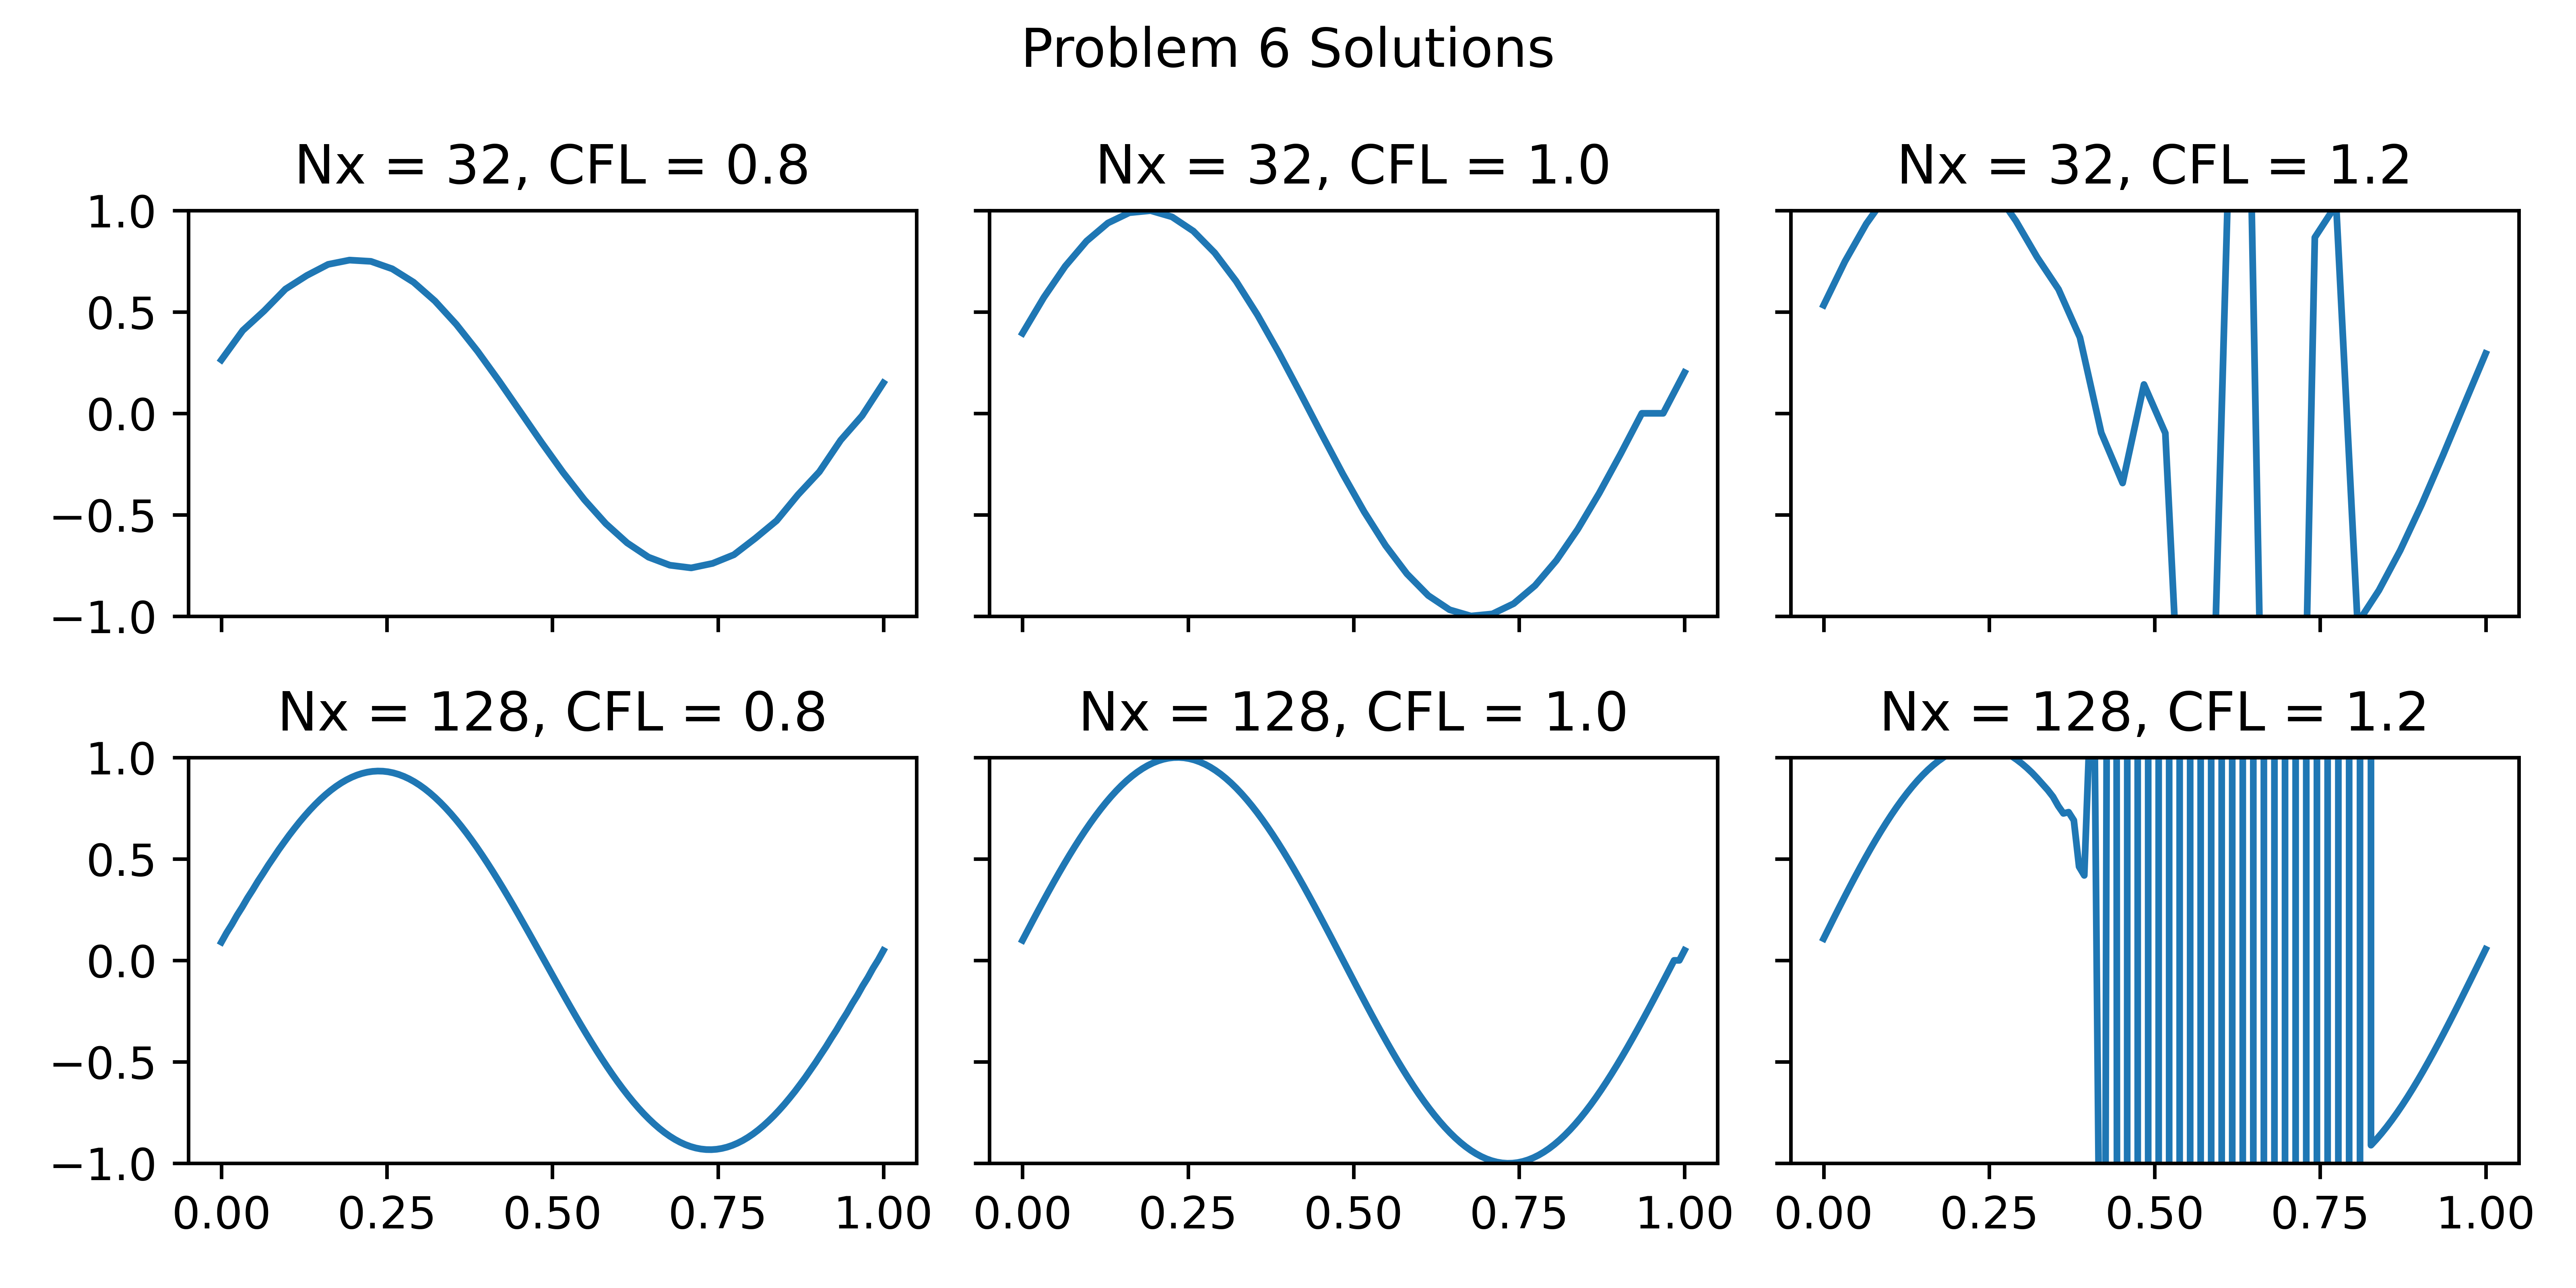
\includegraphics[width=.6\textwidth]{../code/prob6_tstop.png}
    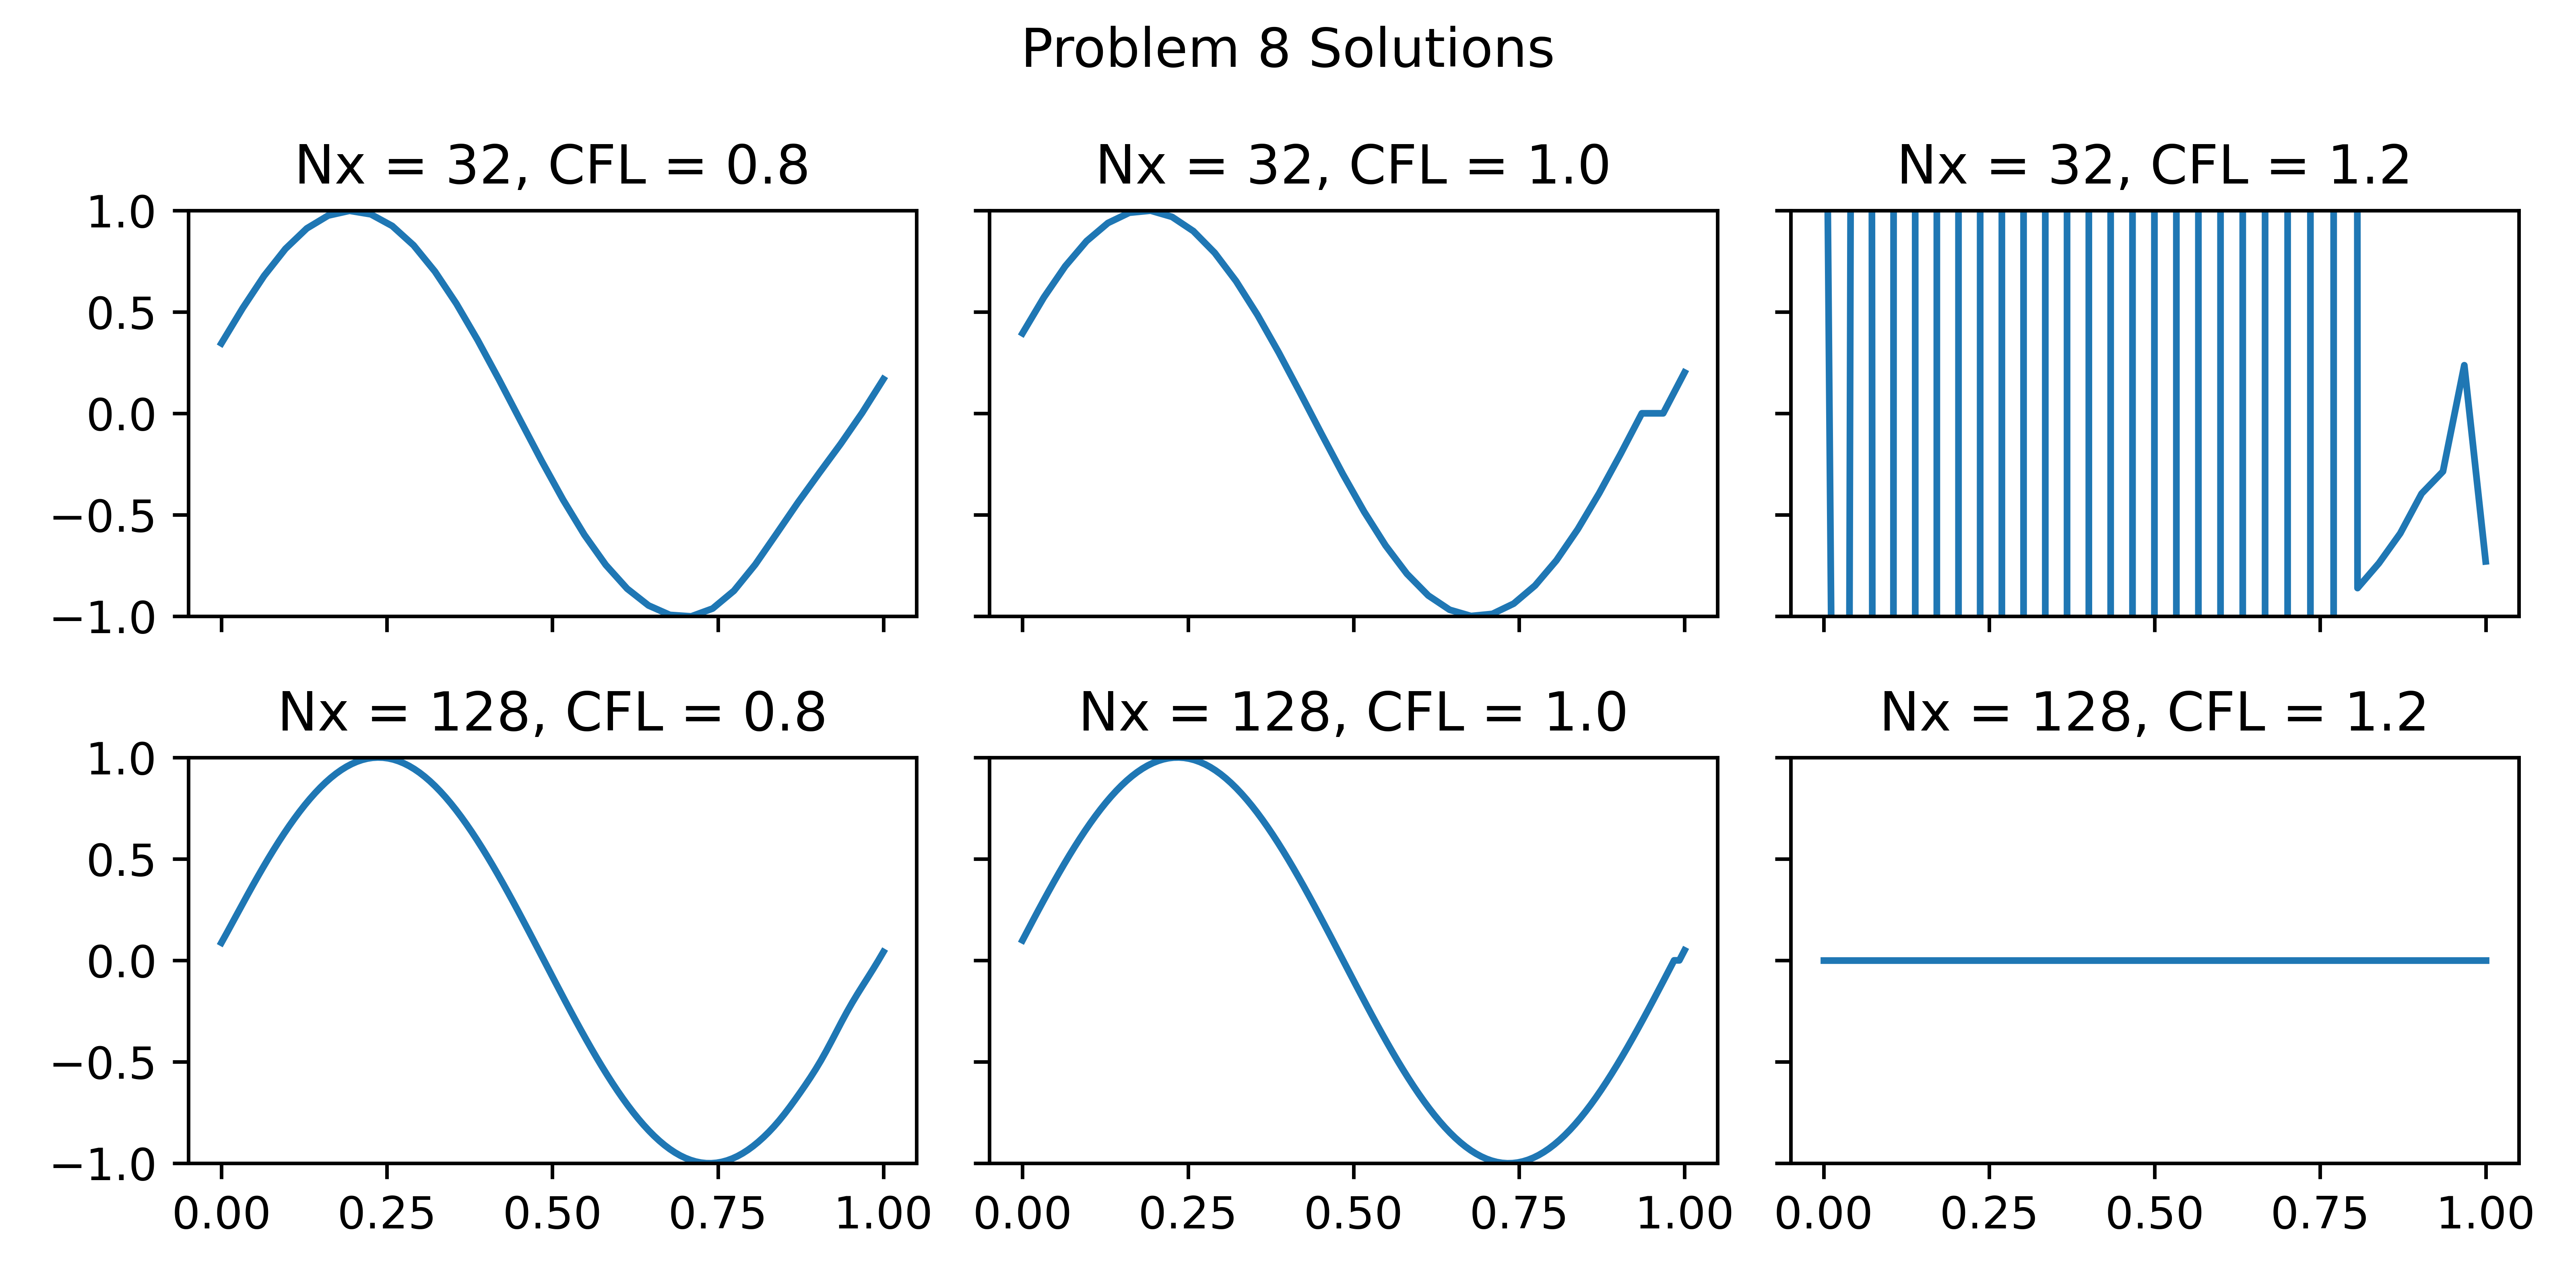
\includegraphics[width=.6\textwidth]{../code/prob8_tstop.png}
    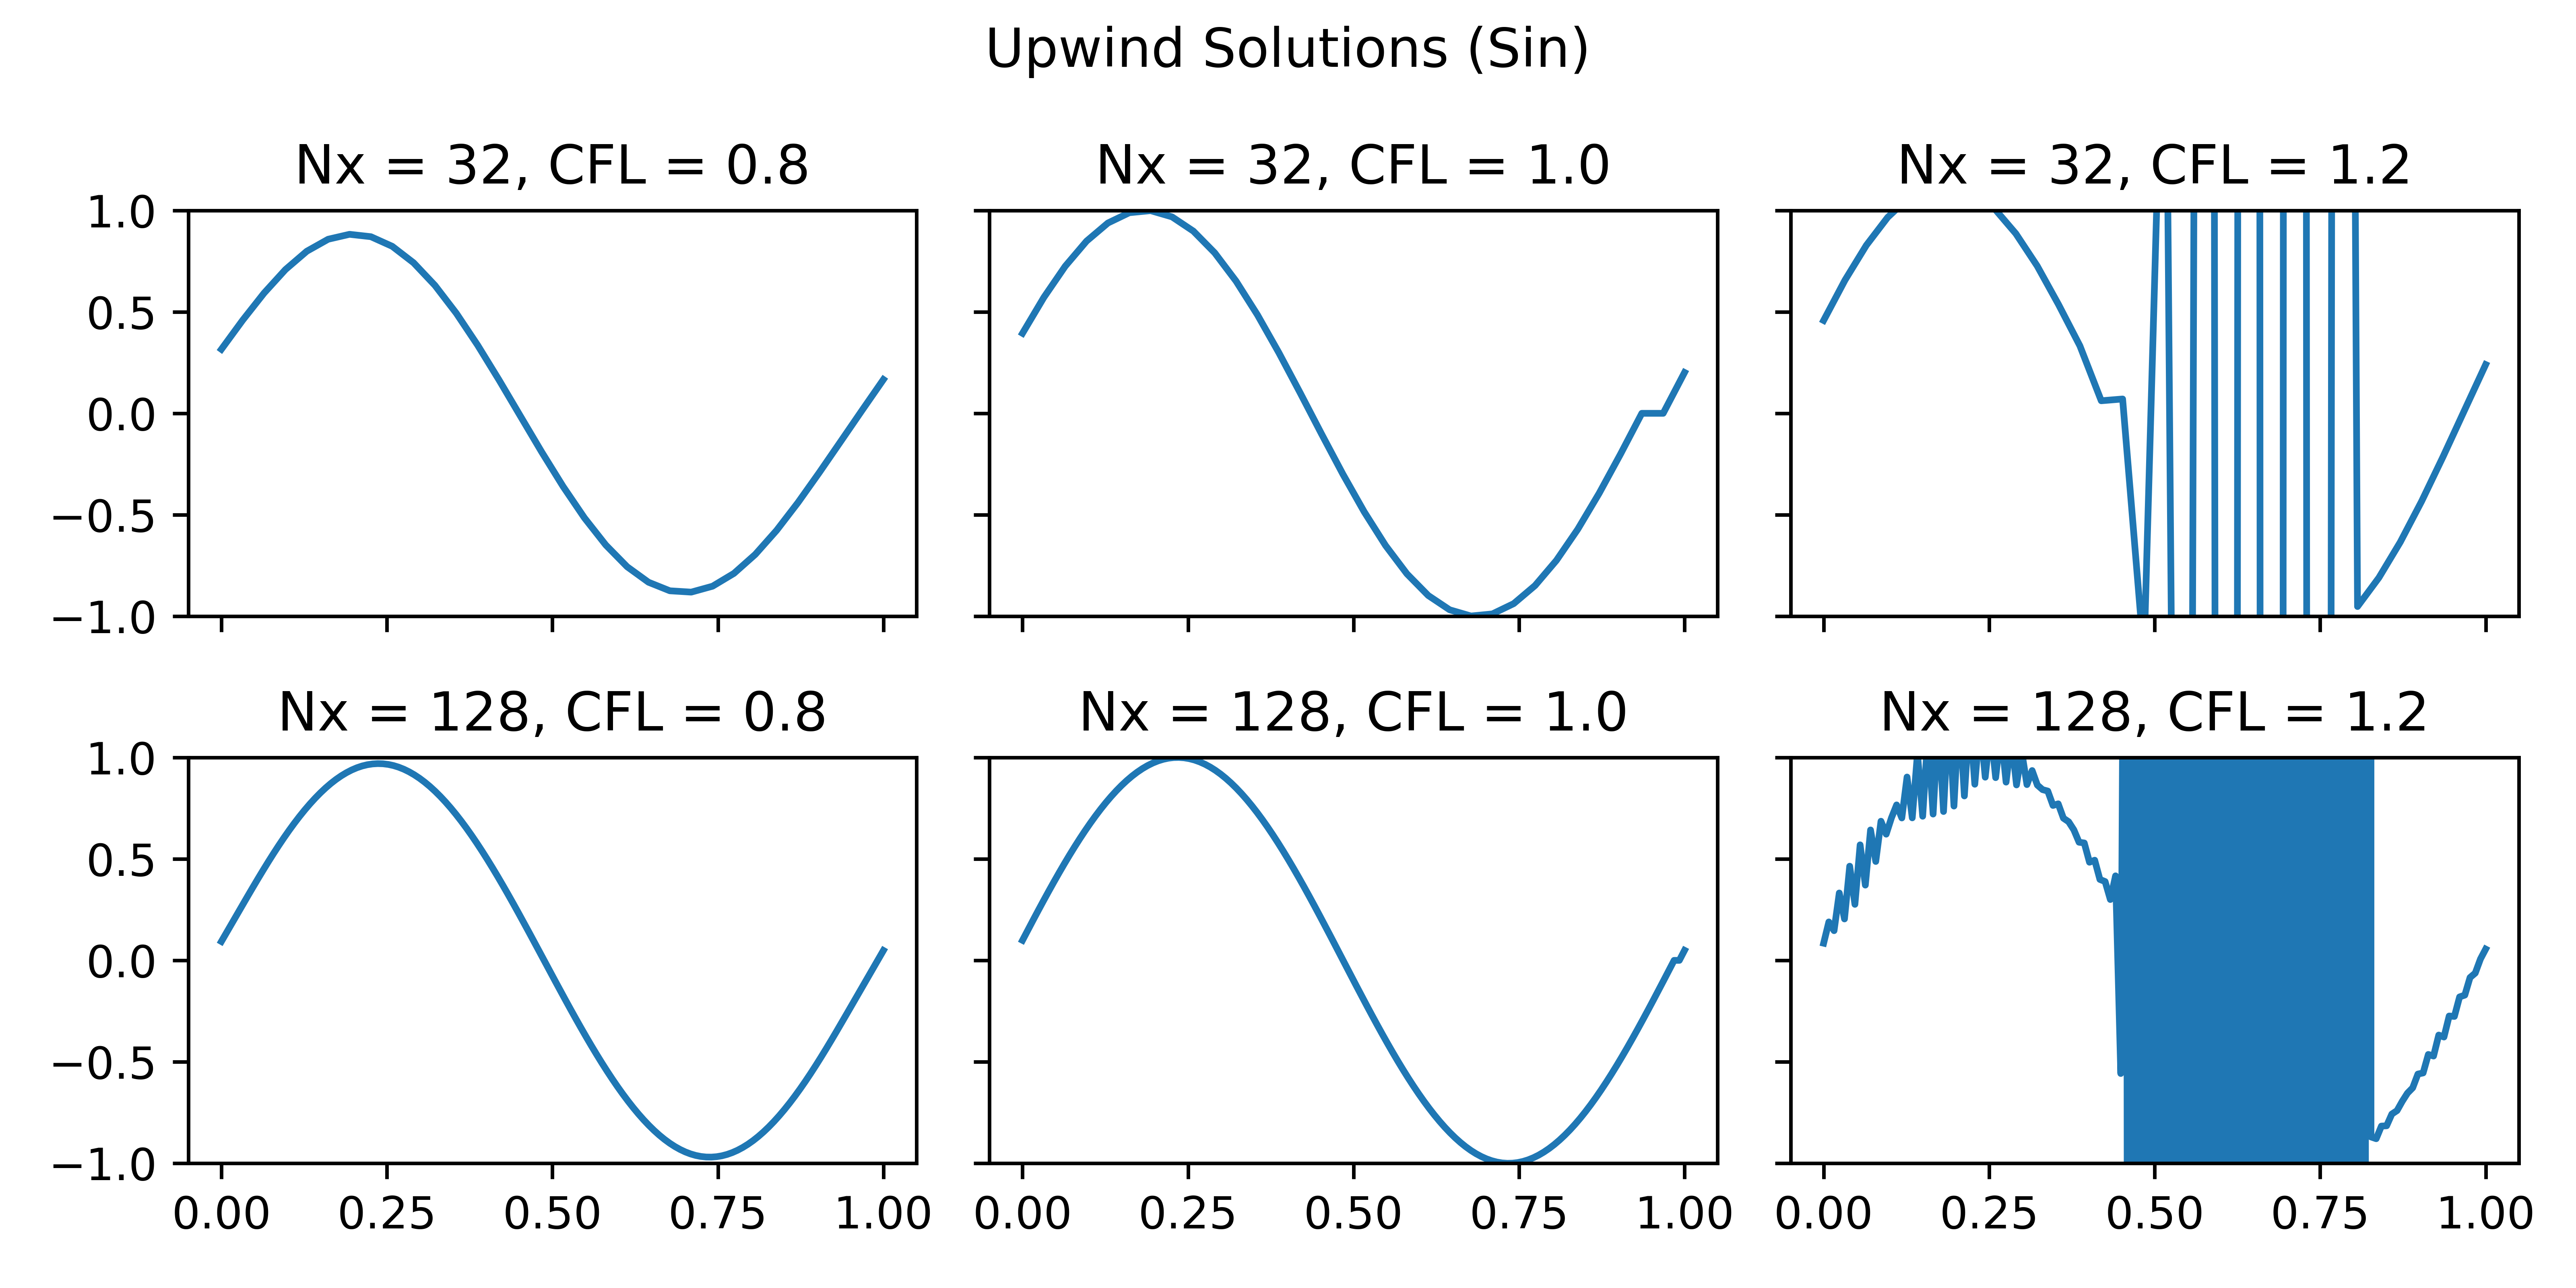
\includegraphics[width=.6\textwidth]{../code/upwind_sin_tstop.png}
    \caption{Sharp Discontinuous IC advected by Lax-Friedrichs Method (a),
    Lax-Wendroff Method (b), and Upwind Method (c) for various grid sizes and
    CFL numbers.}
    \label{fig:sin_adv}
\end{figure}

\section{Discontinuous IC with LF}

\begin{figure}[t]
    \centering
    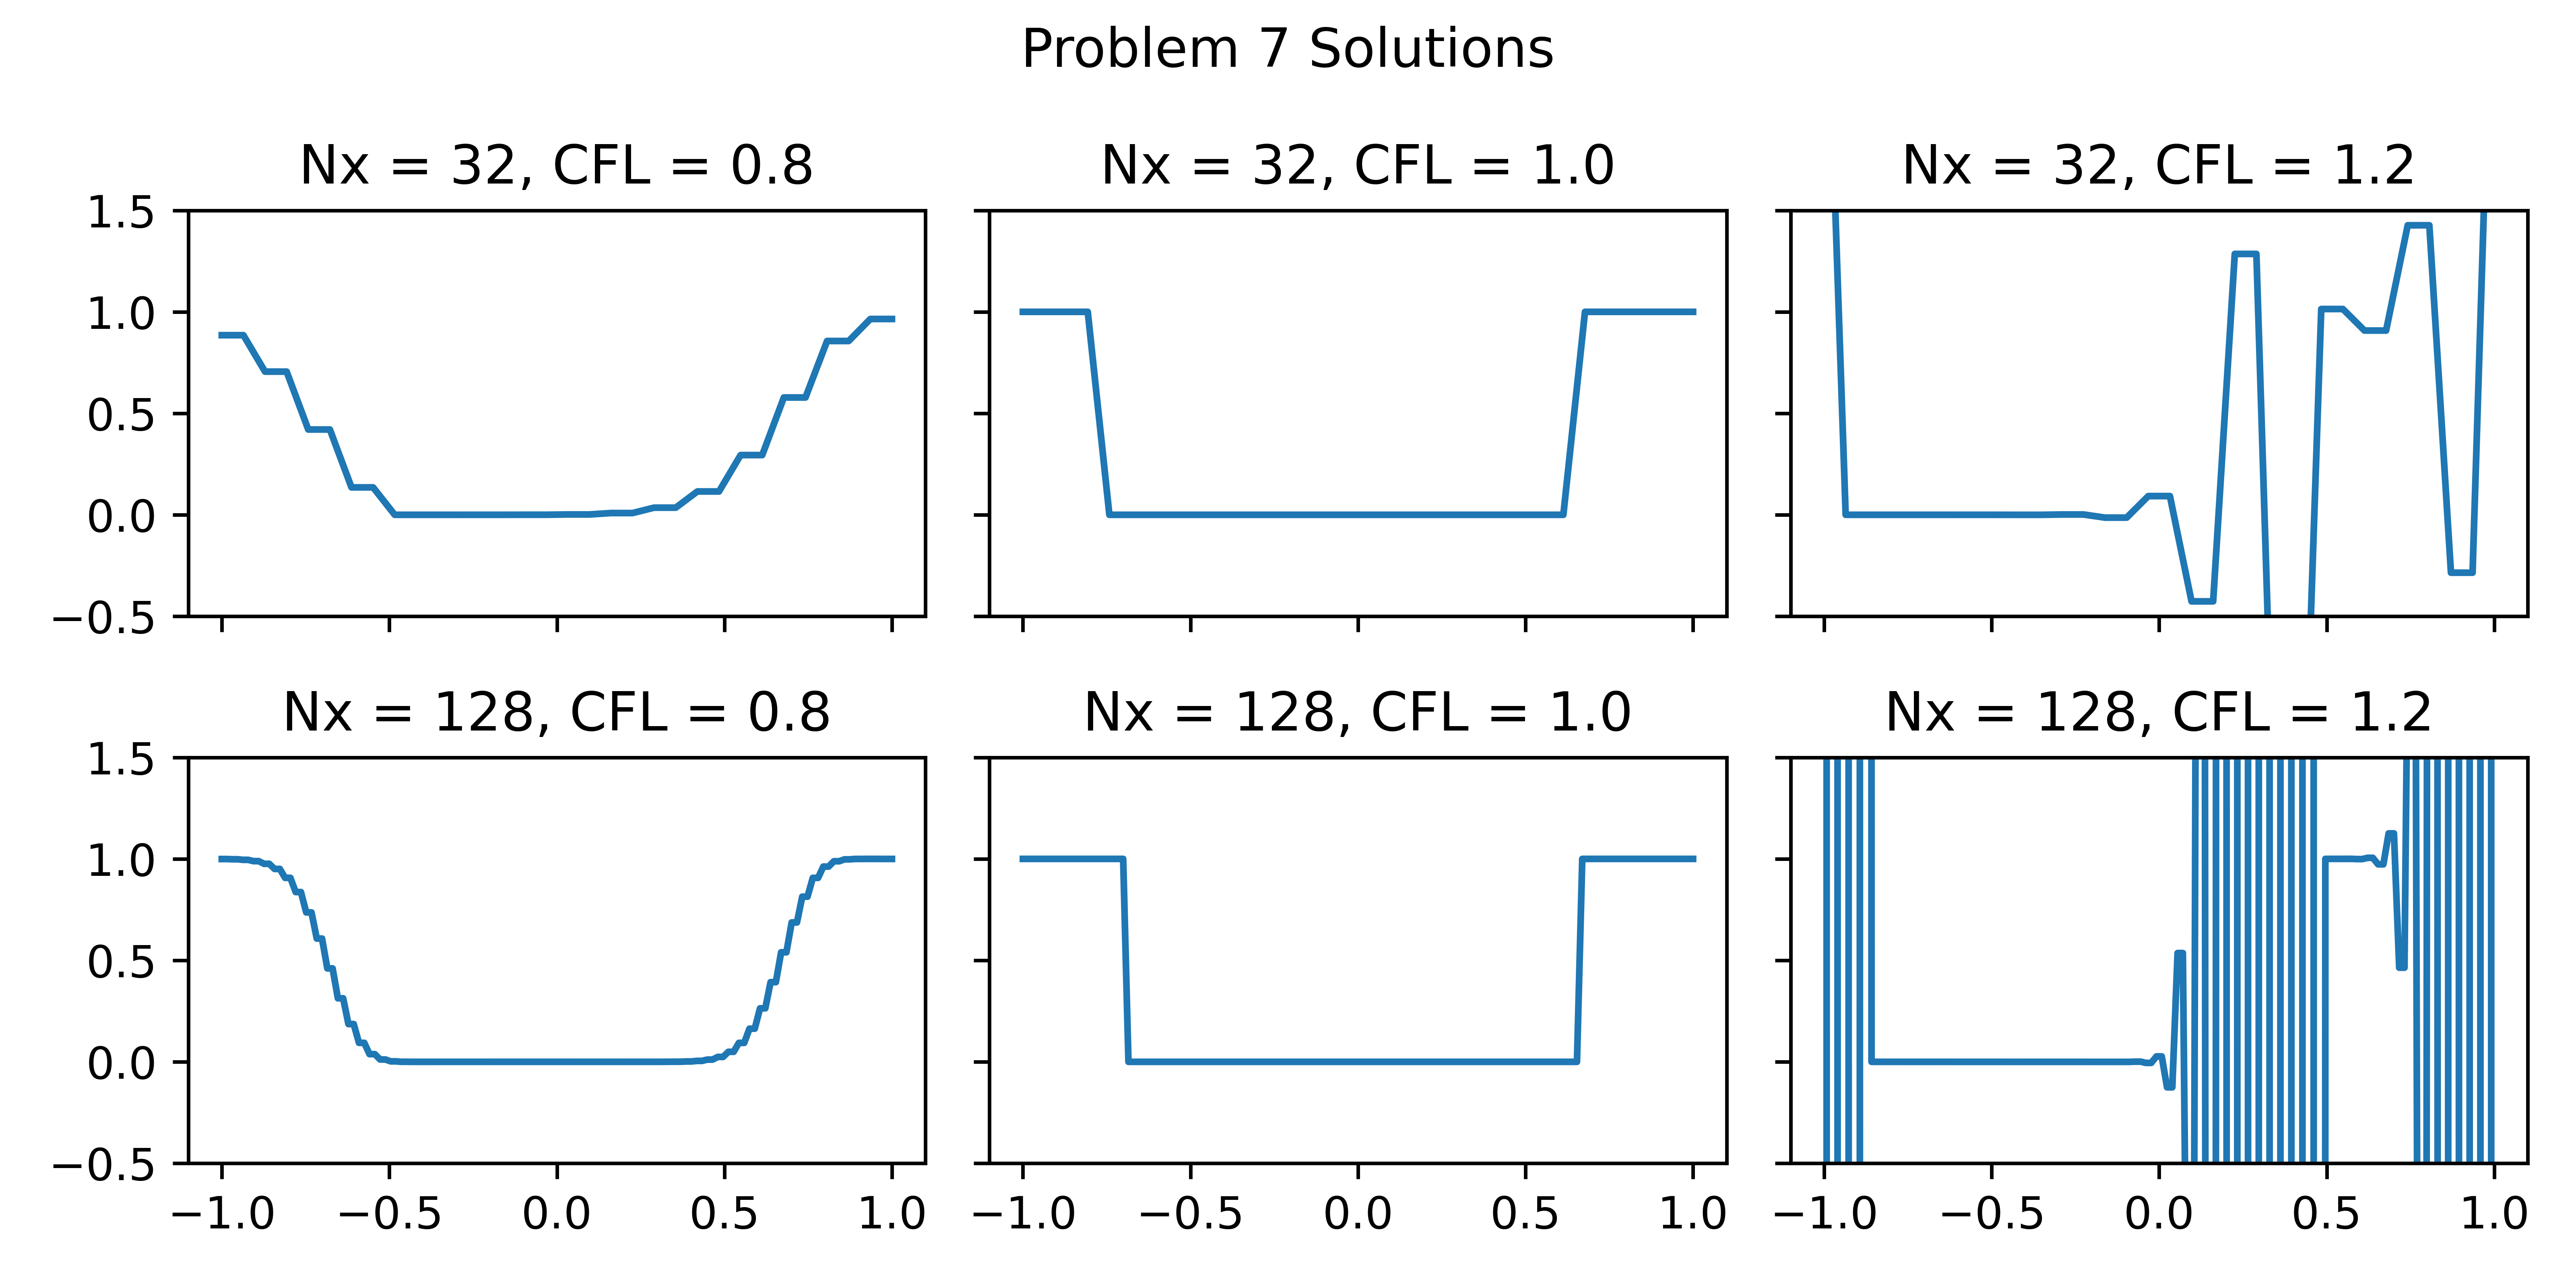
\includegraphics[width=.6\textwidth]{../code/prob7_tstop.png}
    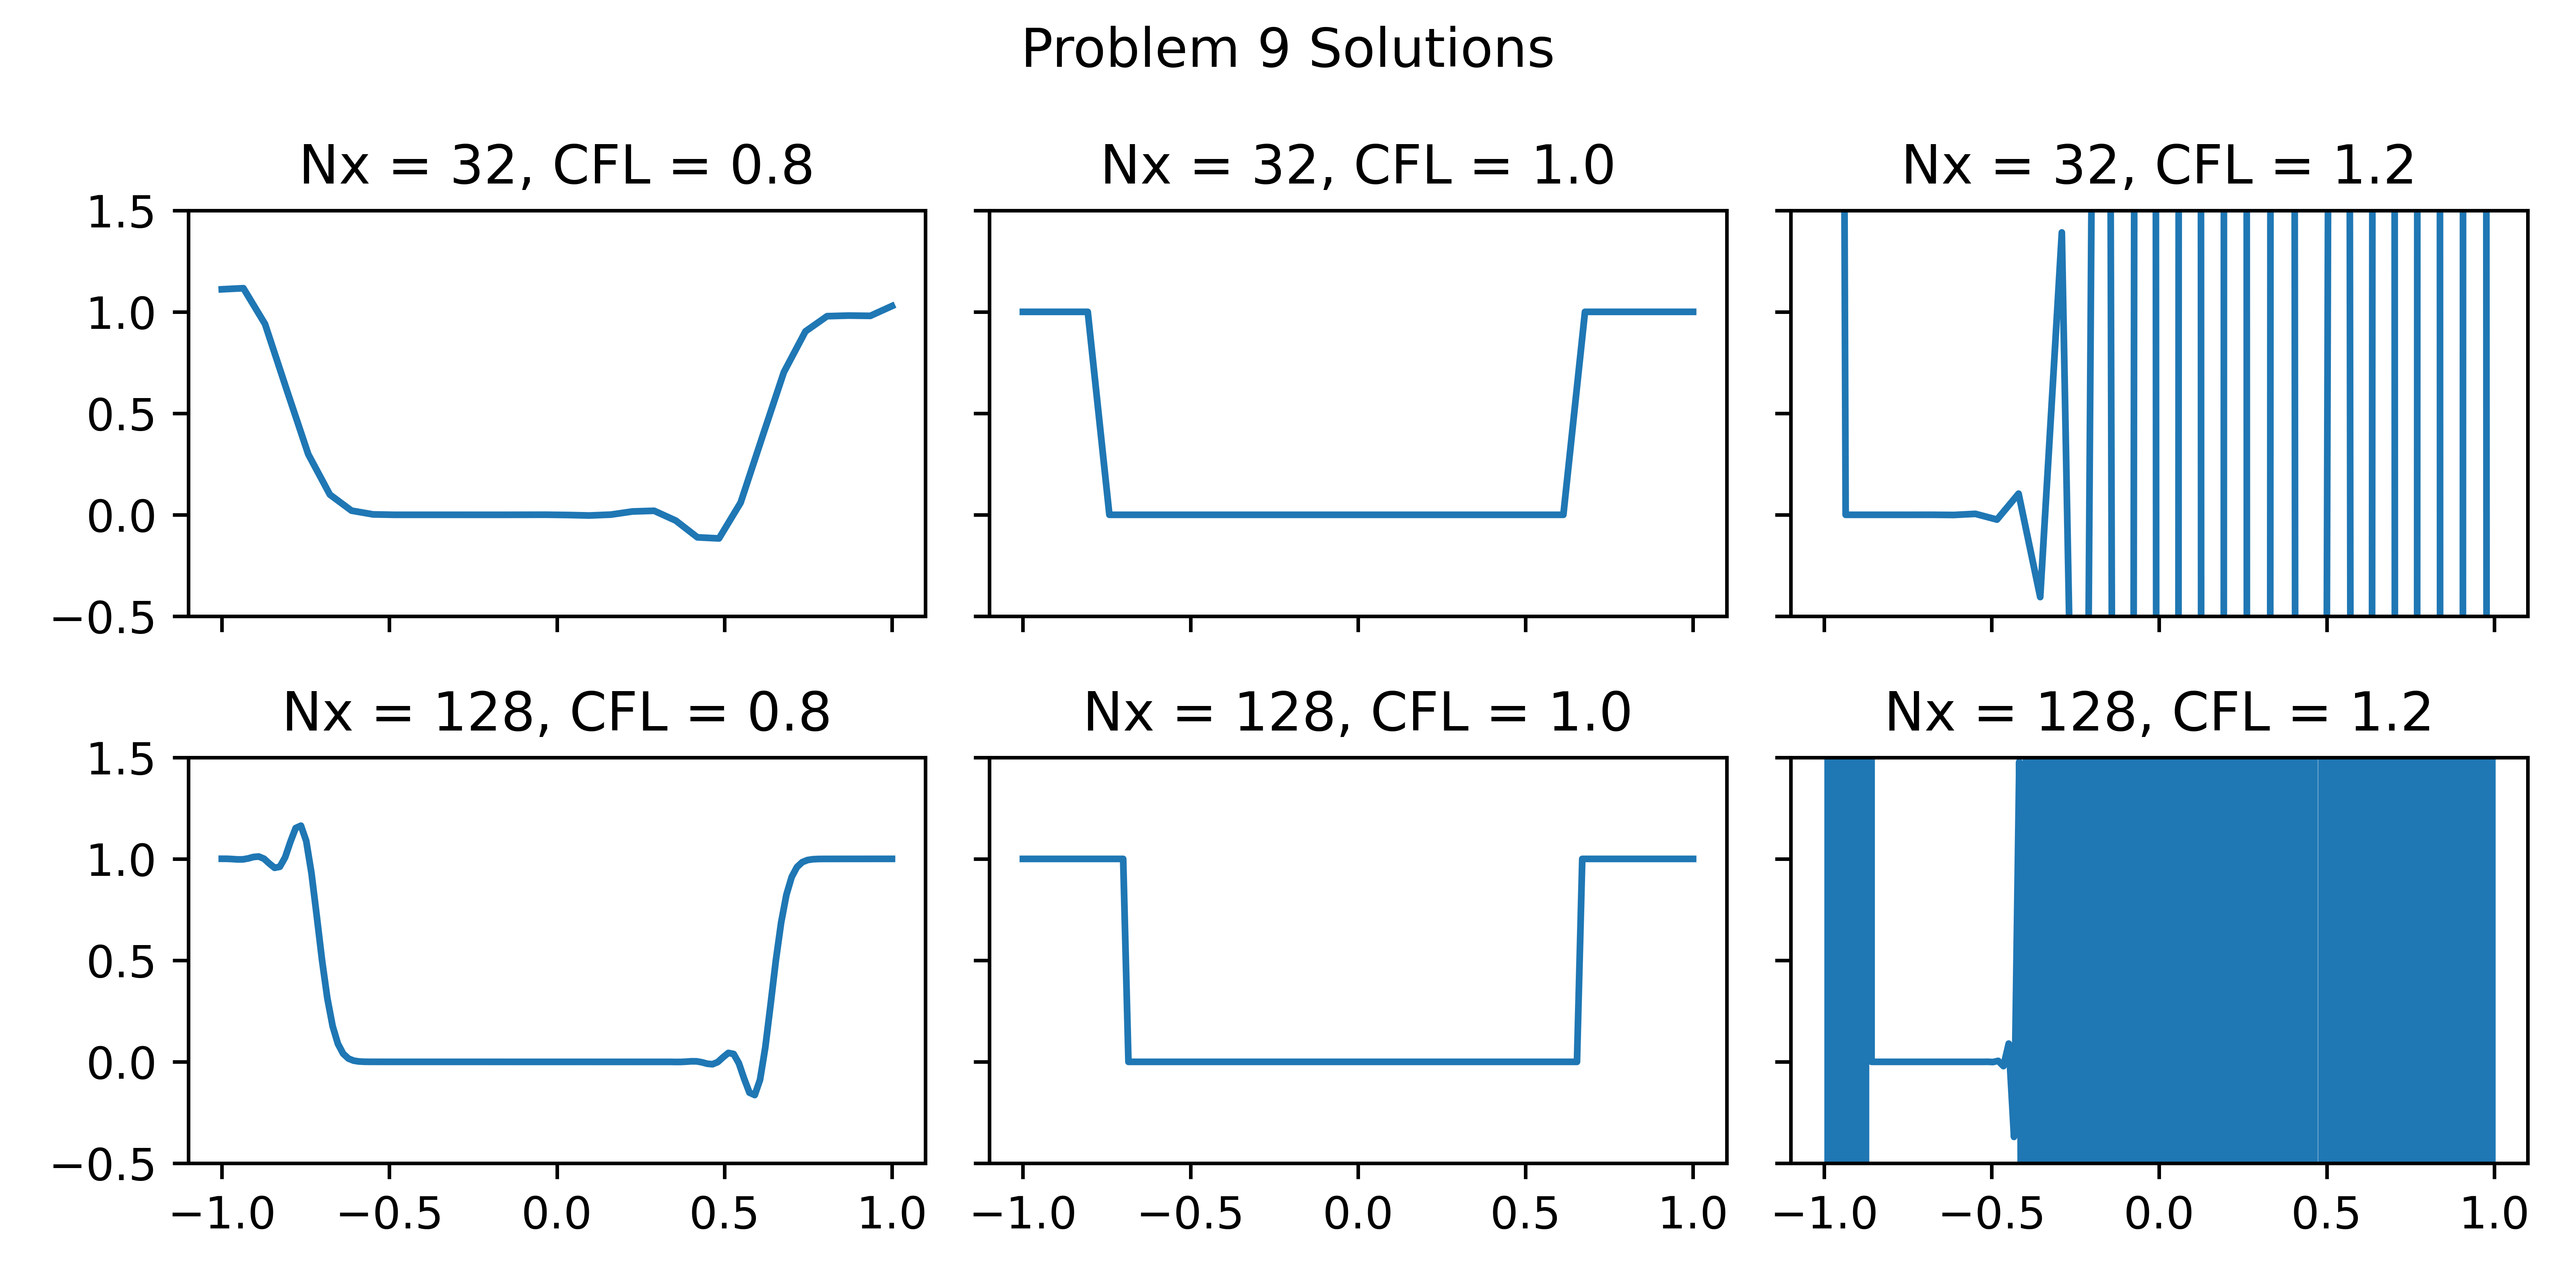
\includegraphics[width=.6\textwidth]{../code/prob9_tstop.png}
    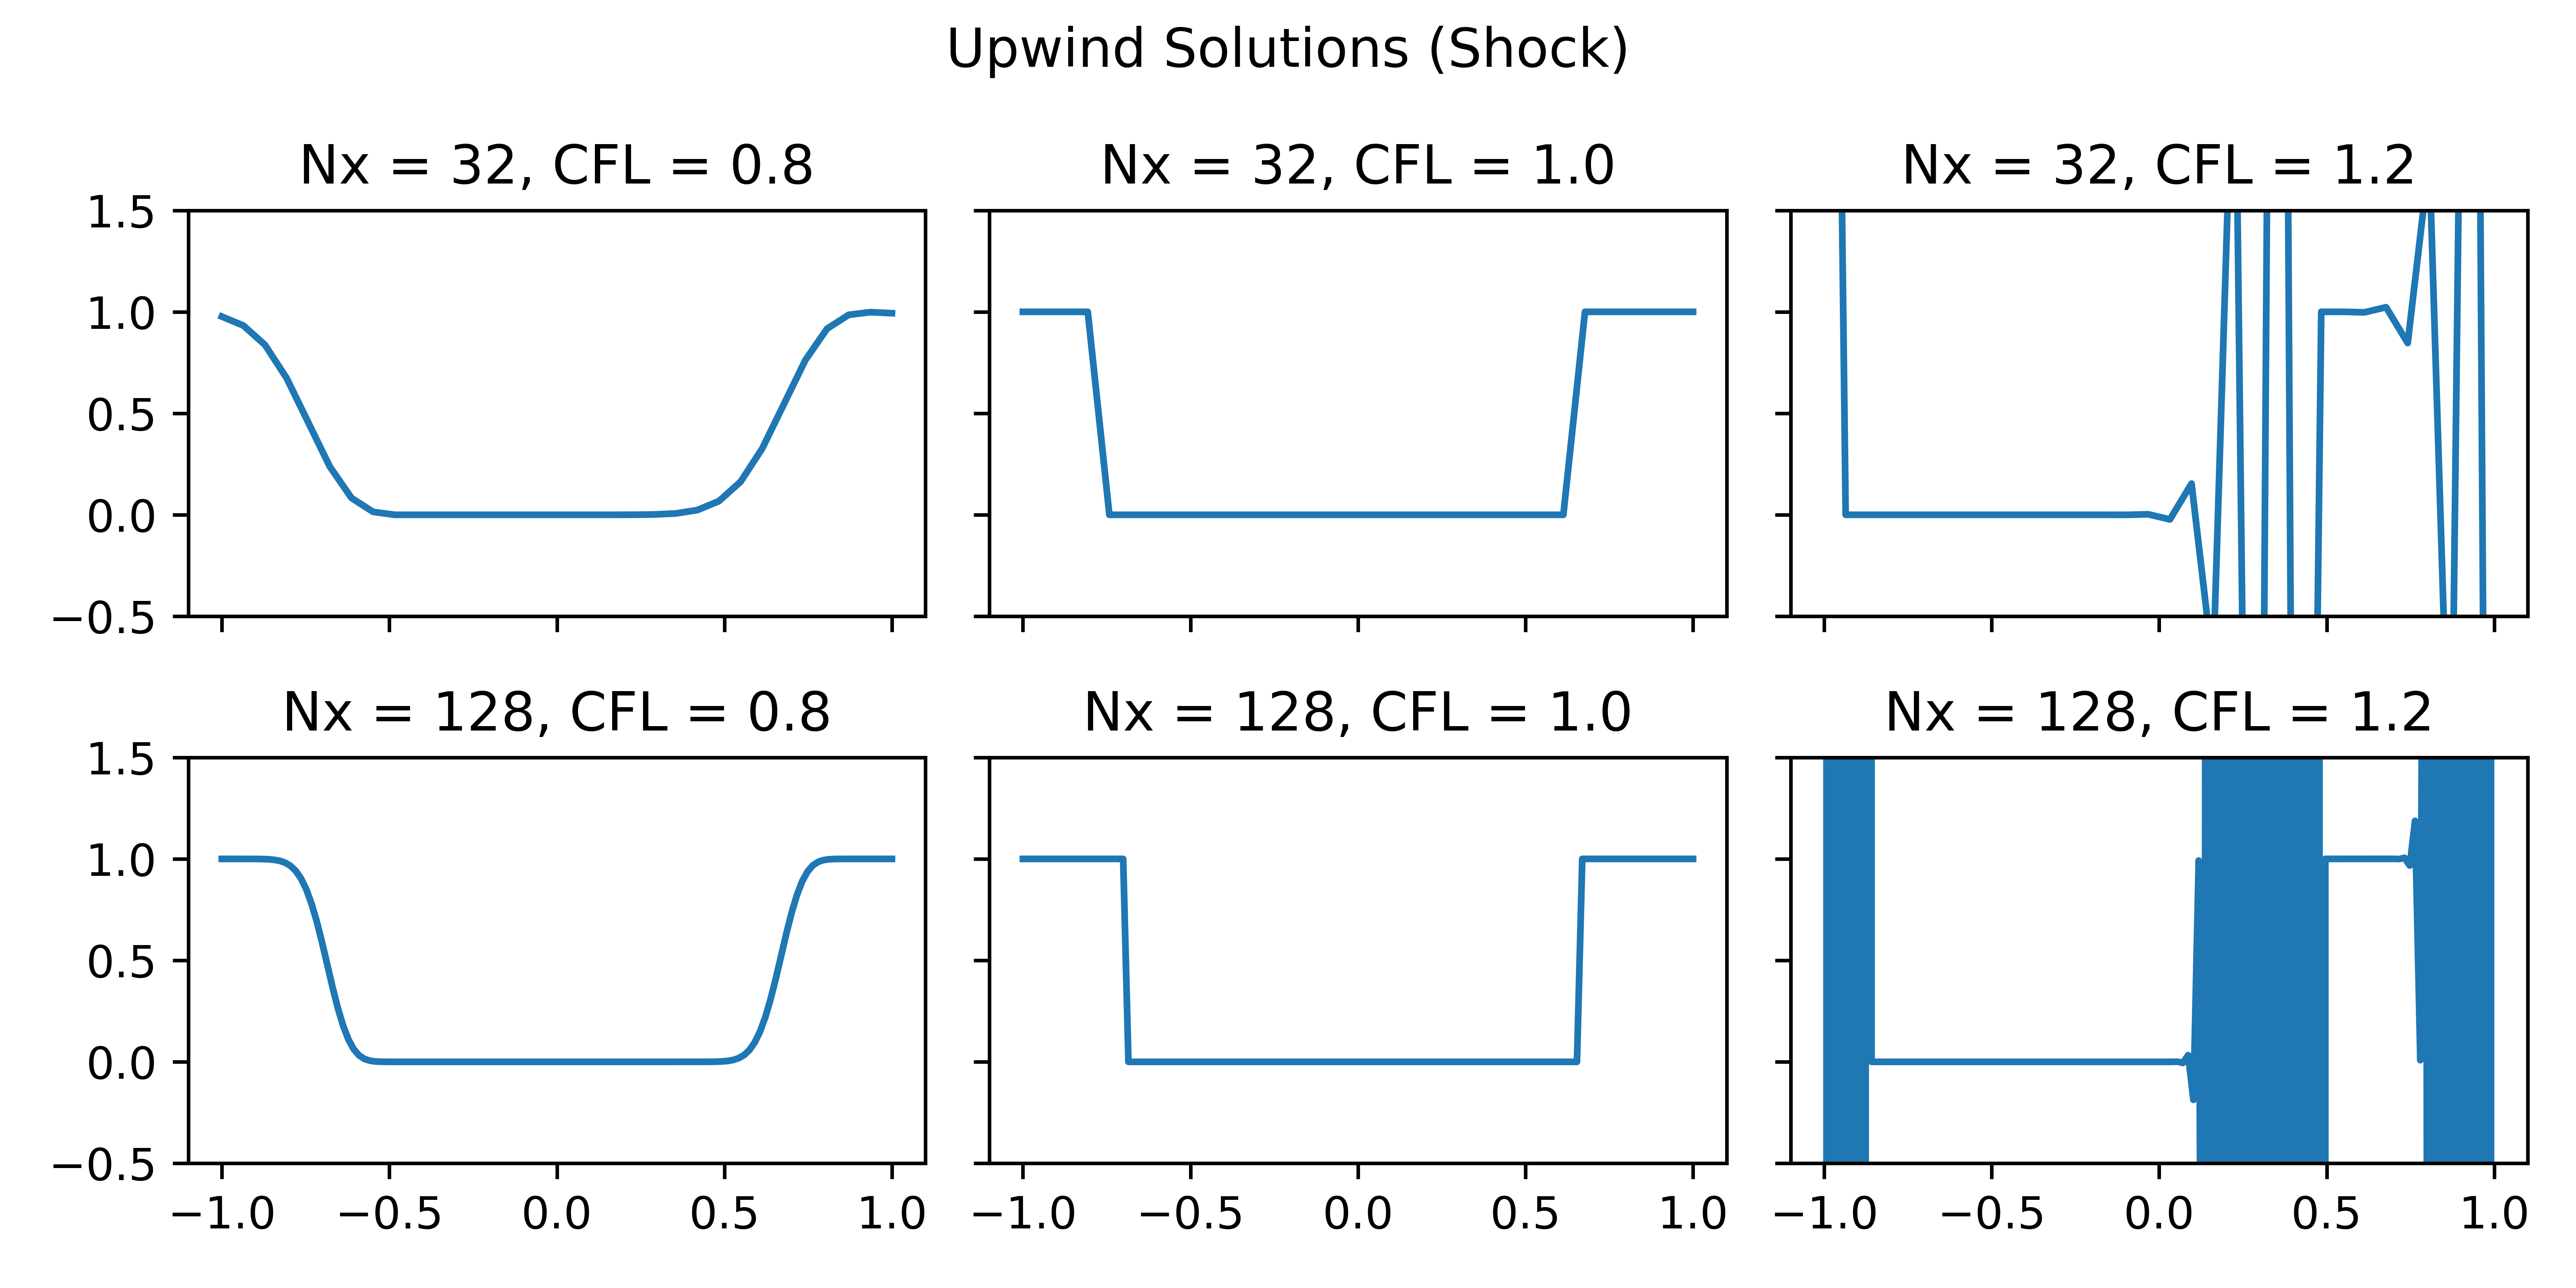
\includegraphics[width=.6\textwidth]{../code/upwind_shock_tstop.png}
    \caption{Sharp Discontinuous IC advected by Lax-Friedrichs Method (a),
    Lax-Wendroff Method (b), and Upwind Method (c) for various grid sizes and
    CFL numbers.}
    \label{fig:discont_ic}
\end{figure}

\section{Sinusoidal Adv. with LW}

\section{Discontinuous IC with LW}


\end{document}
